\documentclass{beamer}\usepackage[]{graphicx}\usepackage[]{color}
%% maxwidth is the original width if it is less than linewidth
%% otherwise use linewidth (to make sure the graphics do not exceed the margin)
\makeatletter
\def\maxwidth{ %
  \ifdim\Gin@nat@width>\linewidth
    \linewidth
  \else
    \Gin@nat@width
  \fi
}
\makeatother

\definecolor{fgcolor}{rgb}{0.345, 0.345, 0.345}
\newcommand{\hlnum}[1]{\textcolor[rgb]{0.686,0.059,0.569}{#1}}%
\newcommand{\hlstr}[1]{\textcolor[rgb]{0.192,0.494,0.8}{#1}}%
\newcommand{\hlcom}[1]{\textcolor[rgb]{0.678,0.584,0.686}{\textit{#1}}}%
\newcommand{\hlopt}[1]{\textcolor[rgb]{0,0,0}{#1}}%
\newcommand{\hlstd}[1]{\textcolor[rgb]{0.345,0.345,0.345}{#1}}%
\newcommand{\hlkwa}[1]{\textcolor[rgb]{0.161,0.373,0.58}{\textbf{#1}}}%
\newcommand{\hlkwb}[1]{\textcolor[rgb]{0.69,0.353,0.396}{#1}}%
\newcommand{\hlkwc}[1]{\textcolor[rgb]{0.333,0.667,0.333}{#1}}%
\newcommand{\hlkwd}[1]{\textcolor[rgb]{0.737,0.353,0.396}{\textbf{#1}}}%
\let\hlipl\hlkwb

\usepackage{framed}
\makeatletter
\newenvironment{kframe}{%
 \def\at@end@of@kframe{}%
 \ifinner\ifhmode%
  \def\at@end@of@kframe{\end{minipage}}%
  \begin{minipage}{\columnwidth}%
 \fi\fi%
 \def\FrameCommand##1{\hskip\@totalleftmargin \hskip-\fboxsep
 \colorbox{shadecolor}{##1}\hskip-\fboxsep
     % There is no \\@totalrightmargin, so:
     \hskip-\linewidth \hskip-\@totalleftmargin \hskip\columnwidth}%
 \MakeFramed {\advance\hsize-\width
   \@totalleftmargin\z@ \linewidth\hsize
   \@setminipage}}%
 {\par\unskip\endMakeFramed%
 \at@end@of@kframe}
\makeatother

\definecolor{shadecolor}{rgb}{.97, .97, .97}
\definecolor{messagecolor}{rgb}{0, 0, 0}
\definecolor{warningcolor}{rgb}{1, 0, 1}
\definecolor{errorcolor}{rgb}{1, 0, 0}
\newenvironment{knitrout}{}{} % an empty environment to be redefined in TeX

\usepackage{alltt}
\IfFileExists{upquote.sty}{\usepackage{upquote}}{}
\begin{document}

\title{A Christmas Carol - Comparison Barplots}
\author{Dayana Moncada}

\begin{frame}
  \titlepage
\end{frame}

\begin{frame}
  \frametitle{Outline}
    \tableofcontents
\end{frame}

\section{Install and Load Libraries}
\begin{frame}[fragile]
  \frametitle{Install and Load Libraries}
    \begin{itemize}
      \item
\begin{knitrout}
\definecolor{shadecolor}{rgb}{0.969, 0.969, 0.969}\color{fgcolor}\begin{kframe}
\begin{alltt}
\hlkwd{library}\hlstd{(dplyr)}
\end{alltt}
\end{kframe}
\end{knitrout}
      \item
\begin{knitrout}
\definecolor{shadecolor}{rgb}{0.969, 0.969, 0.969}\color{fgcolor}\begin{kframe}
\begin{alltt}
\hlkwd{library}\hlstd{(tidytext)}
\end{alltt}
\end{kframe}
\end{knitrout}
    \item
\begin{knitrout}
\definecolor{shadecolor}{rgb}{0.969, 0.969, 0.969}\color{fgcolor}\begin{kframe}
\begin{alltt}
\hlkwd{library}\hlstd{(gutenbergr)}
\end{alltt}
\end{kframe}
\end{knitrout}
    \item
\begin{knitrout}
\definecolor{shadecolor}{rgb}{0.969, 0.969, 0.969}\color{fgcolor}\begin{kframe}
\begin{alltt}
\hlkwd{library}\hlstd{(ggplot2)}
\end{alltt}
\end{kframe}
\end{knitrout}
    \item
\begin{knitrout}
\definecolor{shadecolor}{rgb}{0.969, 0.969, 0.969}\color{fgcolor}\begin{kframe}
\begin{alltt}
\hlkwd{library}\hlstd{(stringr)}
\end{alltt}
\end{kframe}
\end{knitrout}
    
    \end{itemize}
\end{frame}

\section{Access Project Gutenberg}
\begin{frame}[fragile]
  \frametitle{Access Project Gutenberg}
\begin{knitrout}
\definecolor{shadecolor}{rgb}{0.969, 0.969, 0.969}\color{fgcolor}\begin{kframe}
\begin{alltt}
\hlstd{df}\hlkwb{<-}\hlkwd{gutenberg_works}\hlstd{(}\hlkwd{str_detect}\hlstd{(title,}\hlstr{'A Christmas Carol'}\hlstd{))}
\hlstd{df}\hlopt{$}\hlstd{gutenberg_id}
\end{alltt}
\begin{verbatim}
## [1]    46 19337 30368 40729 41739
\end{verbatim}
\begin{alltt}
\hlstd{df}\hlopt{$}\hlstd{title}
\end{alltt}
\begin{verbatim}
## [1] "A Christmas Carol in Prose; Being a Ghost Story of Christmas"                                                      
## [2] "A Christmas Carol"                                                                                                 
## [3] "A Christmas Carol\nThe original manuscript"                                                                        
## [4] "\"Old Scrooge\": A Christmas Carol in Five Staves.\r\nDramatized from Charles Dickens' Celebrated Christmas Story."
## [5] "A Christmas Carol; Or, The Miser's Warning!\r\n(Adapted from Charles Dickens' Celebrated Work.)"
\end{verbatim}
\end{kframe}
\end{knitrout}
\end{frame}

\section{Download Carol}
\begin{frame}[fragile]
  \frametitle{Download Carol}
\begin{knitrout}
\definecolor{shadecolor}{rgb}{0.969, 0.969, 0.969}\color{fgcolor}\begin{kframe}
\begin{alltt}
\hlstd{carol}\hlkwb{<-}\hlkwd{gutenberg_download}\hlstd{(}\hlnum{46}\hlstd{)}
\end{alltt}
\end{kframe}
\end{knitrout}
\end{frame}

\section{Unpack the Words}
\begin{frame}[fragile]
  \frametitle{Unpack the Words}
\begin{knitrout}
\definecolor{shadecolor}{rgb}{0.969, 0.969, 0.969}\color{fgcolor}\begin{kframe}
\begin{alltt}
\hlstd{carol_words}\hlkwb{<-}\hlstd{carol}\hlopt
  \hlkwd{unnest_tokens}\hlstd{(word,text)}
\hlkwd{colnames}\hlstd{(carol_words)}
\end{alltt}
\begin{verbatim}
## [1] "gutenberg_id" "word"
\end{verbatim}
\end{kframe}
\end{knitrout}
\end{frame}

\section{The Bing Lexicon}
\begin{frame}[fragile]
  \frametitle{The Bing Lexicon}
\begin{knitrout}
\definecolor{shadecolor}{rgb}{0.969, 0.969, 0.969}\color{fgcolor}\begin{kframe}
\begin{alltt}
  \hlstd{bing}\hlkwb{<-}\hlkwd{get_sentiments}\hlstd{(}\hlstr{'bing'}\hlstd{)}
  \hlkwd{colnames}\hlstd{(bing)}
\end{alltt}
\begin{verbatim}
## [1] "word"      "sentiment"
\end{verbatim}
\begin{alltt}
  \hlstd{bing[}\hlnum{498}\hlopt{:}\hlnum{500}\hlstd{,]}
\end{alltt}
\begin{verbatim}
## # A tibble: 3 x 2
##          word sentiment
##         <chr>     <chr>
## 1     bereave  negative
## 2 bereavement  negative
## 3      bereft  negative
\end{verbatim}
\end{kframe}
\end{knitrout}
\end{frame}

\section{The Inner Join}
\begin{frame}[fragile]
  \frametitle{The Inner Join}
\begin{knitrout}
\definecolor{shadecolor}{rgb}{0.969, 0.969, 0.969}\color{fgcolor}\begin{kframe}
\begin{alltt}
  \hlstd{carol_words}\hlkwb{<-}\hlkwd{inner_join}\hlstd{(carol_words,bing)}
\end{alltt}


{\ttfamily\noindent\itshape\color{messagecolor}{\#\# Joining, by = "{}word"{}}}\begin{alltt}
  \hlstd{carol_words}\hlopt{$}\hlstd{gutenberg_id}\hlkwb{<-}\hlkwa{NULL}
  \hlstd{carol_words[}\hlnum{498}\hlopt{:}\hlnum{500}\hlstd{,]}
\end{alltt}
\begin{verbatim}
## # A tibble: 3 x 2
##        word sentiment
##       <chr>     <chr>
## 1 strangest  negative
## 2    bright  positive
## 3     clear  positive
\end{verbatim}
\end{kframe}
\end{knitrout}
\end{frame}

\section{Plotting Sentiments}
\begin{frame}[fragile]
  \frametitle{Positive Words}
\begin{knitrout}
\definecolor{shadecolor}{rgb}{0.969, 0.969, 0.969}\color{fgcolor}\begin{kframe}
\begin{alltt}
\hlstd{carol_pos}\hlkwb{<-}\hlstd{carol_words}\hlopt
  \hlkwd{filter}\hlstd{(sentiment}\hlopt{==}\hlstr{'positive'}\hlstd{)}\hlopt
  \hlkwd{group_by}\hlstd{(word)}\hlopt
  \hlkwd{summarize}\hlstd{(}\hlkwc{count}\hlstd{=}\hlkwd{n}\hlstd{(),}\hlkwc{sentiment}\hlstd{=}\hlkwd{first}\hlstd{(sentiment))}\hlopt
  \hlkwd{arrange}\hlstd{(count)}\hlopt
  \hlkwd{top_n}\hlstd{(}\hlnum{10}\hlstd{,}\hlkwc{wt}\hlstd{=count)}

\hlstd{carol_pos}\hlopt{$}\hlstd{word}\hlkwb{<-}\hlkwd{factor}\hlstd{(carol_pos}\hlopt{$}\hlstd{word,}\hlkwc{levels}\hlstd{=carol_pos}\hlopt{$}\hlstd{word)}

\hlkwd{ggplot}\hlstd{()}\hlopt{+}
  \hlkwd{geom_bar}\hlstd{(}\hlkwc{data}\hlstd{=carol_pos,}\hlkwd{aes}\hlstd{(}\hlkwc{x}\hlstd{=word,}\hlkwc{y}\hlstd{=count),}\hlkwc{stat}\hlstd{=}\hlstr{'identity'}\hlstd{)}\hlopt{+}
  \hlkwd{coord_flip}\hlstd{()}
\end{alltt}
\end{kframe}
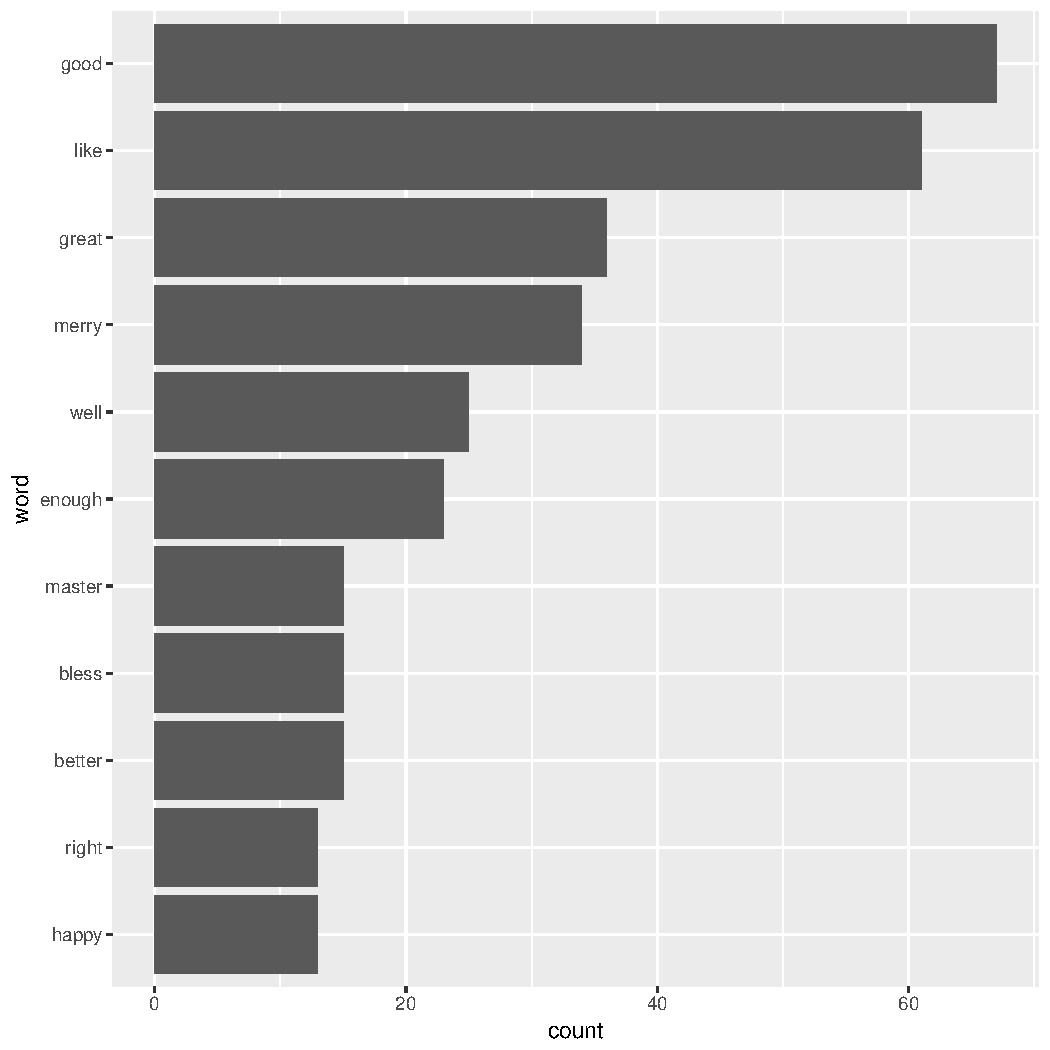
\includegraphics[width=\maxwidth]{figure/unnamed-chunk-11-1} 

\end{knitrout}
\end{frame}
\begin{frame}[fragile]  
  \frametitle{Plotting}
\begin{knitrout}
\definecolor{shadecolor}{rgb}{0.969, 0.969, 0.969}\color{fgcolor}\begin{kframe}
\begin{alltt}
\hlstd{carol_pos}\hlopt{$}\hlstd{word}\hlkwb{<-}\hlkwd{factor}\hlstd{(carol_pos}\hlopt{$}\hlstd{word,}\hlkwc{levels}\hlstd{=carol_pos}\hlopt{$}\hlstd{word)}

\hlkwd{ggplot}\hlstd{()}\hlopt{+}
  \hlkwd{geom_bar}\hlstd{(}\hlkwc{data}\hlstd{=carol_pos,}\hlkwd{aes}\hlstd{(}\hlkwc{x}\hlstd{=word,}\hlkwc{y}\hlstd{=count),}\hlkwc{stat}\hlstd{=}\hlstr{'identity'}\hlstd{)}\hlopt{+}
  \hlkwd{coord_flip}\hlstd{()}
\end{alltt}
\end{kframe}
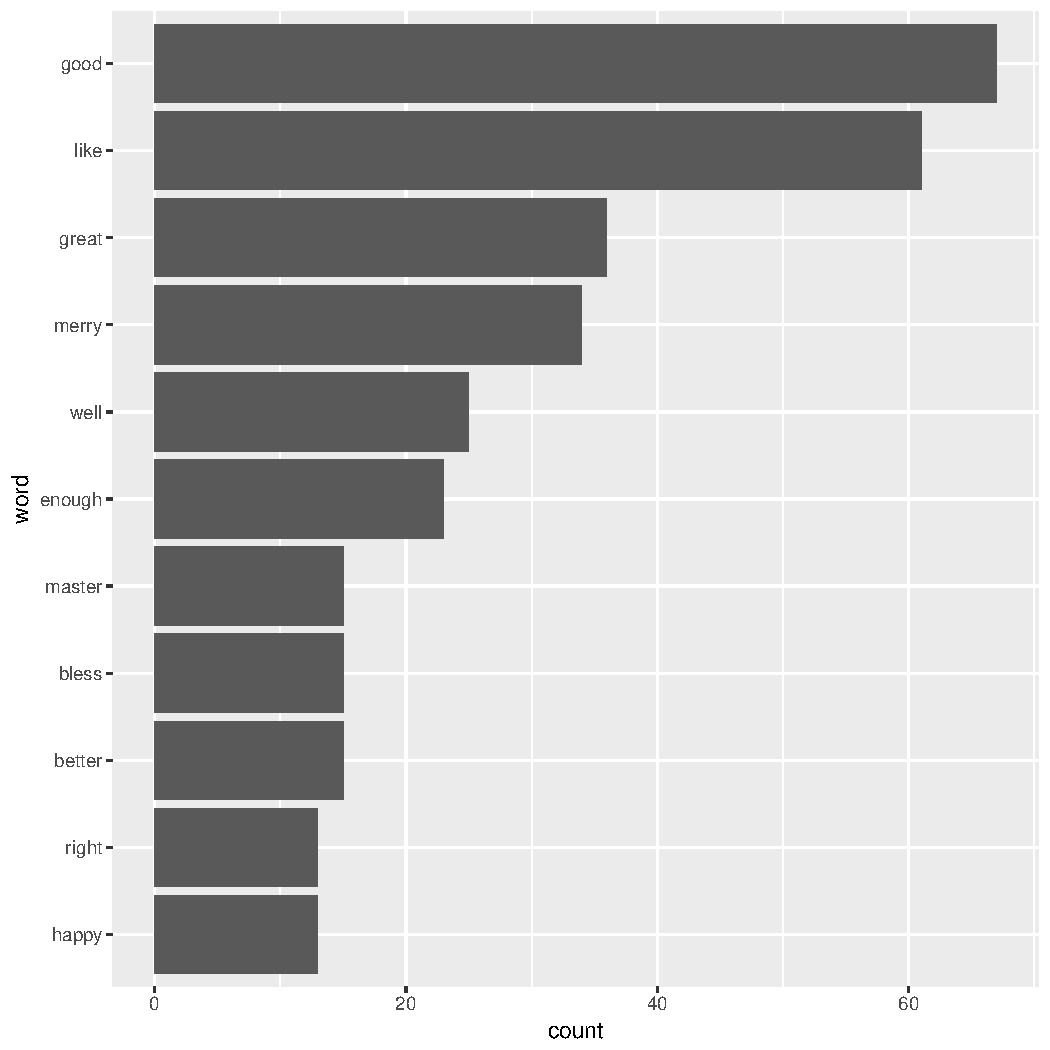
\includegraphics[width=\maxwidth]{figure/unnamed-chunk-12-1} 

\end{knitrout}
\end{frame}

\section{Negative Words}
\begin{frame}[fragile]
  \frametitle{Negative Words}
\begin{knitrout}
\definecolor{shadecolor}{rgb}{0.969, 0.969, 0.969}\color{fgcolor}\begin{kframe}
\begin{alltt}
\hlstd{carol_neg}\hlkwb{<-}\hlstd{carol_words}\hlopt
  \hlkwd{filter}\hlstd{(sentiment}\hlopt{==}\hlstr{'negative'}\hlstd{)}\hlopt
  \hlkwd{group_by}\hlstd{(word)}\hlopt
  \hlkwd{summarize}\hlstd{(}\hlkwc{count}\hlstd{=}\hlkwd{n}\hlstd{(),}\hlkwc{sentiment}\hlstd{=}\hlkwd{first}\hlstd{(sentiment))}\hlopt
  \hlkwd{arrange}\hlstd{(count)}\hlopt
  \hlkwd{filter}\hlstd{(word} \hlopt{!=} \hlstr{'miss'}\hlstd{)}\hlopt
  \hlkwd{top_n}\hlstd{(}\hlnum{10}\hlstd{,}\hlkwc{wt}\hlstd{=count)}
\end{alltt}
\end{kframe}
\end{knitrout}
\end{frame}

\begin{frame}[fragile]
  \frametitle{Plotting}
\begin{knitrout}
\definecolor{shadecolor}{rgb}{0.969, 0.969, 0.969}\color{fgcolor}\begin{kframe}
\begin{alltt}
\hlstd{carol_neg}\hlopt{$}\hlstd{word}\hlkwb{<-}\hlkwd{factor}\hlstd{(carol_neg}\hlopt{$}\hlstd{word,}\hlkwc{levels}\hlstd{=carol_neg}\hlopt{$}\hlstd{word)}

\hlkwd{ggplot}\hlstd{()}\hlopt{+}
  \hlkwd{geom_bar}\hlstd{(}\hlkwc{data}\hlstd{=carol_neg,}\hlkwd{aes}\hlstd{(}\hlkwc{x}\hlstd{=word,}\hlkwc{y}\hlstd{=count),}\hlkwc{stat}\hlstd{=}\hlstr{'identity'}\hlstd{)}\hlopt{+}
  \hlkwd{coord_flip}\hlstd{()}
\end{alltt}
\end{kframe}
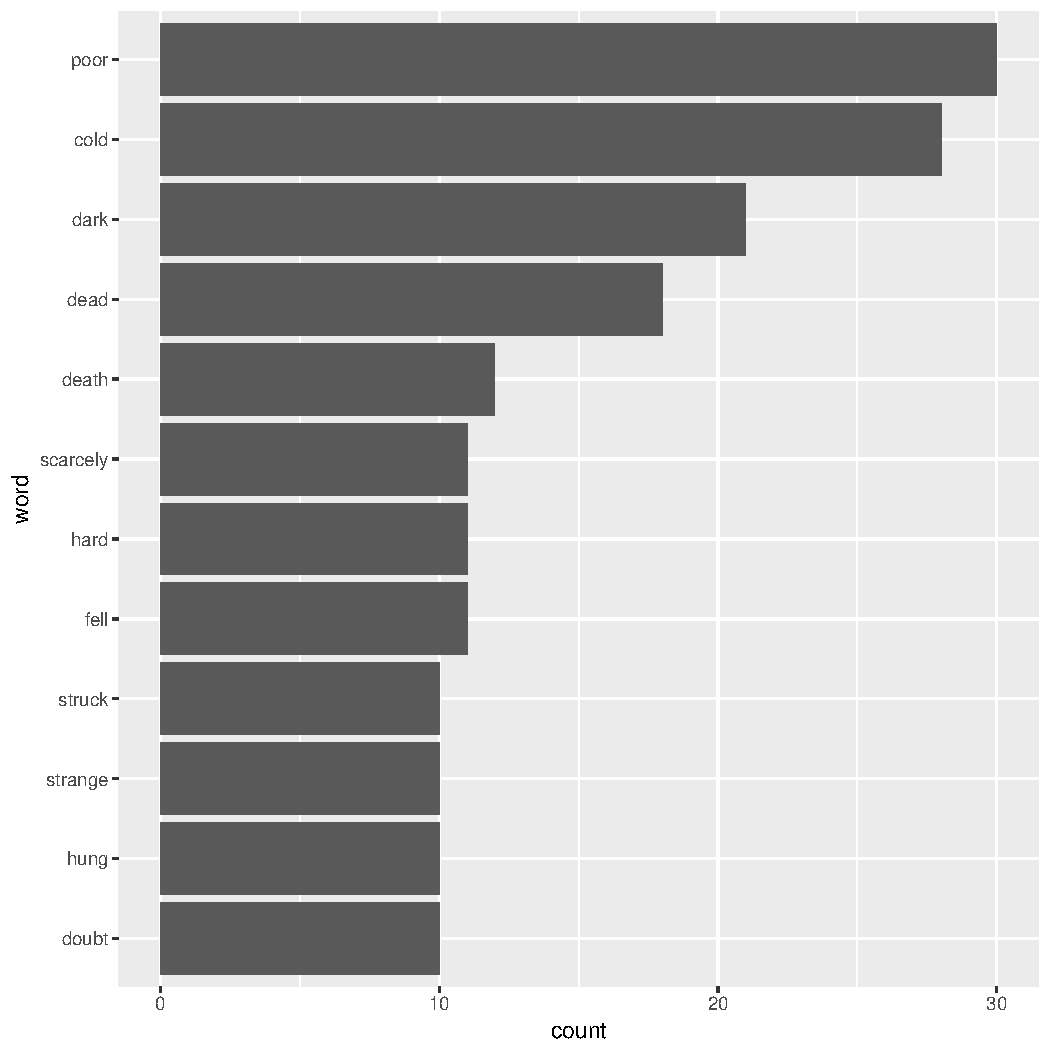
\includegraphics[width=\maxwidth]{figure/unnamed-chunk-14-1} 

\end{knitrout}
\end{frame}


\section{Comparison Plot}
\begin{frame}[fragile]
  \frametitle{Comparison Plot}
\begin{knitrout}
\definecolor{shadecolor}{rgb}{0.969, 0.969, 0.969}\color{fgcolor}\begin{kframe}
\begin{alltt}
\hlstd{carol_comp}\hlkwb{<-}\hlkwd{rbind}\hlstd{(carol_pos,carol_neg)}

\hlkwd{ggplot}\hlstd{()}\hlopt{+}
  \hlkwd{geom_bar}\hlstd{(}\hlkwc{data}\hlstd{=carol_comp,}\hlkwd{aes}\hlstd{(}\hlkwc{x}\hlstd{=word,}\hlkwc{y}\hlstd{=count,}
                               \hlkwc{fill}\hlstd{=sentiment,} \hlkwc{color}\hlstd{=sentiment),}\hlkwc{stat}\hlstd{=}\hlstr{'identity'}\hlstd{)}\hlopt{+}
  \hlkwd{coord_flip}\hlstd{()}\hlopt{+}
  \hlkwd{facet_wrap}\hlstd{(}\hlopt{~}\hlstd{sentiment,}\hlkwc{scales}\hlstd{=}\hlstr{'free_y'}\hlstd{)}\hlopt{+}
  \hlkwd{scale_fill_manual}\hlstd{(}\hlkwc{values}\hlstd{=}\hlkwd{c}\hlstd{(}\hlstr{'green'}\hlstd{,}\hlstr{'red'}\hlstd{))}\hlopt{+}
\hlkwd{scale_color_manual}\hlstd{(}\hlkwc{values}\hlstd{=}\hlkwd{c}\hlstd{(}\hlstr{'green'}\hlstd{,}\hlstr{'red'}\hlstd{))}
\end{alltt}
\end{kframe}
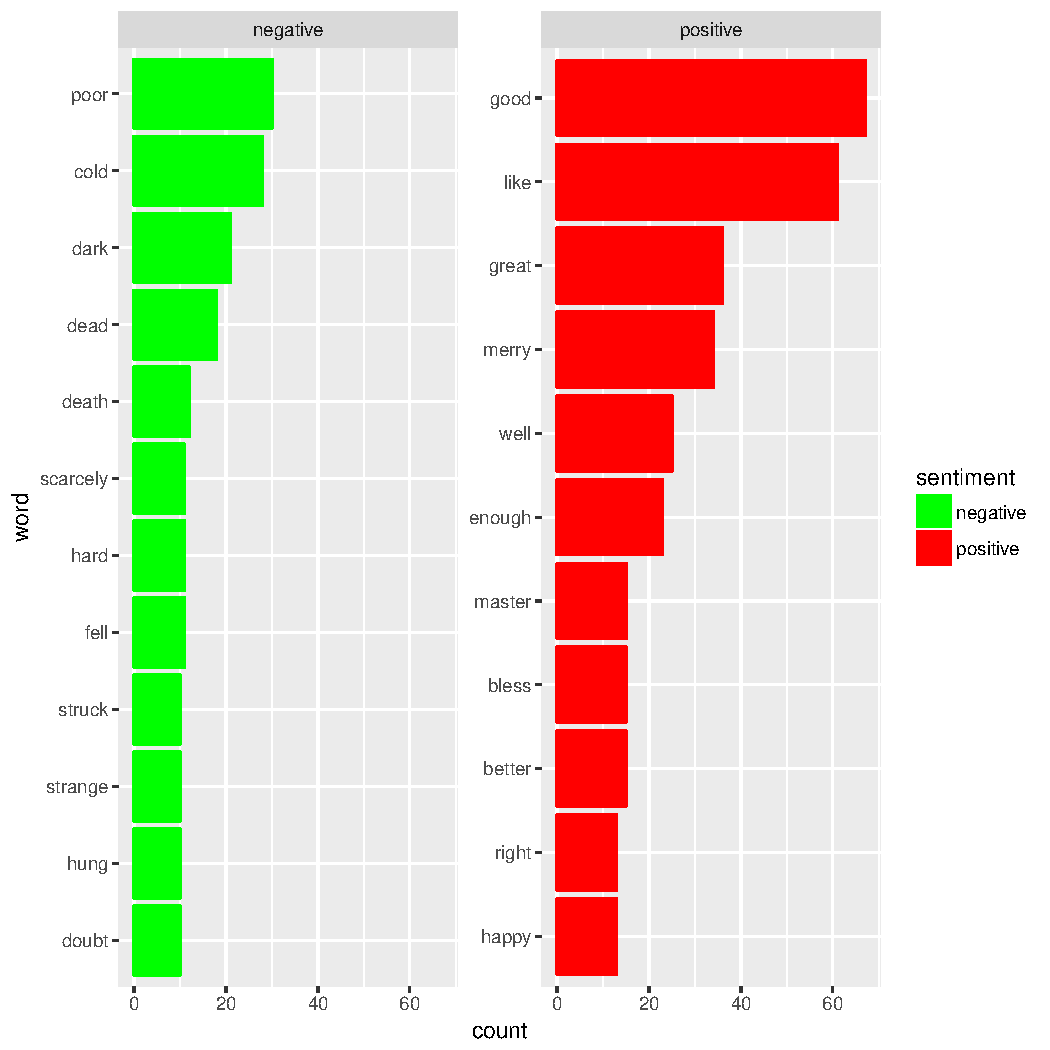
\includegraphics[width=\maxwidth]{figure/unnamed-chunk-15-1} 

\end{knitrout}

\end{frame}
\end{document}
